% =====================================================================
\chapter{Evaluación}
\label{cap:evaluacion}

Este capítulo corresponde a la quinta fase de CRISP-DM: los resultados en el test, del 02/02/2026
al 29/04/2026, que ningún modelo vio al entrenar; las pruebas de robustez; la verificación con la
econometría clásica; y el veredicto sobre la hipótesis.

% ---------------------------------------------------------------------
\section{Noticias \flecha{} precio}
\label{sec:res-np}

\textbf{Las noticias no mejoran la predicción del precio.} Los dos modelos quedan apenas por encima
del azar (tabla~\ref{tab:res-np}): con regresión logística, el modelo A, solo con datos del
mercado, obtiene un AUC de \dato{np.m.logistica.A.auc@3}, y el modelo B, con noticias,
\dato{np.m.logistica.B.auc@3}. La diferencia es
$\Delta\text{AUC} = \dato{np.d.logistica.delta_auc@s3}$, con un intervalo del 95\% de
[\dato{np.d.logistica.ic95_inf@s3};\ \dato{np.d.logistica.ic95_sup@s3}], que incluye el 0. El
random forest dice lo mismo: $\Delta\text{AUC} = \dato{np.d.random_forest.delta_auc@s3}$
[\dato{np.d.random_forest.ic95_inf@s3};\ \dato{np.d.random_forest.ic95_sup@s3}]. Predecir si una
acción sube mañana es difícil con cualquier información diaria, y el sentimiento de las noticias
no agrega nada a lo que ya dicen los retornos, el volumen y el VIX.

\begin{table}[H]
\centering\small
\begin{tabular}{@{}llcccc@{}}
\toprule
\textbf{Algoritmo} & \textbf{Modelo} & \textbf{AUC} & \textbf{Balanced acc.} & \textbf{F1} & \textbf{Exactitud} \\
\midrule
\tabla{metricas_np}
\bottomrule
\end{tabular}
\caption{Noticias \flecha{} precio: métricas en el test (\dato{np.filas_test} filas). Modelo A: solo
mercado; modelo B: mercado más noticias. Fuente: elaboración propia
(\carpeta{4_modelado/noticias_a_precio}).}
\label{tab:res-np}
\end{table}

\begin{figure}[H]
\centering
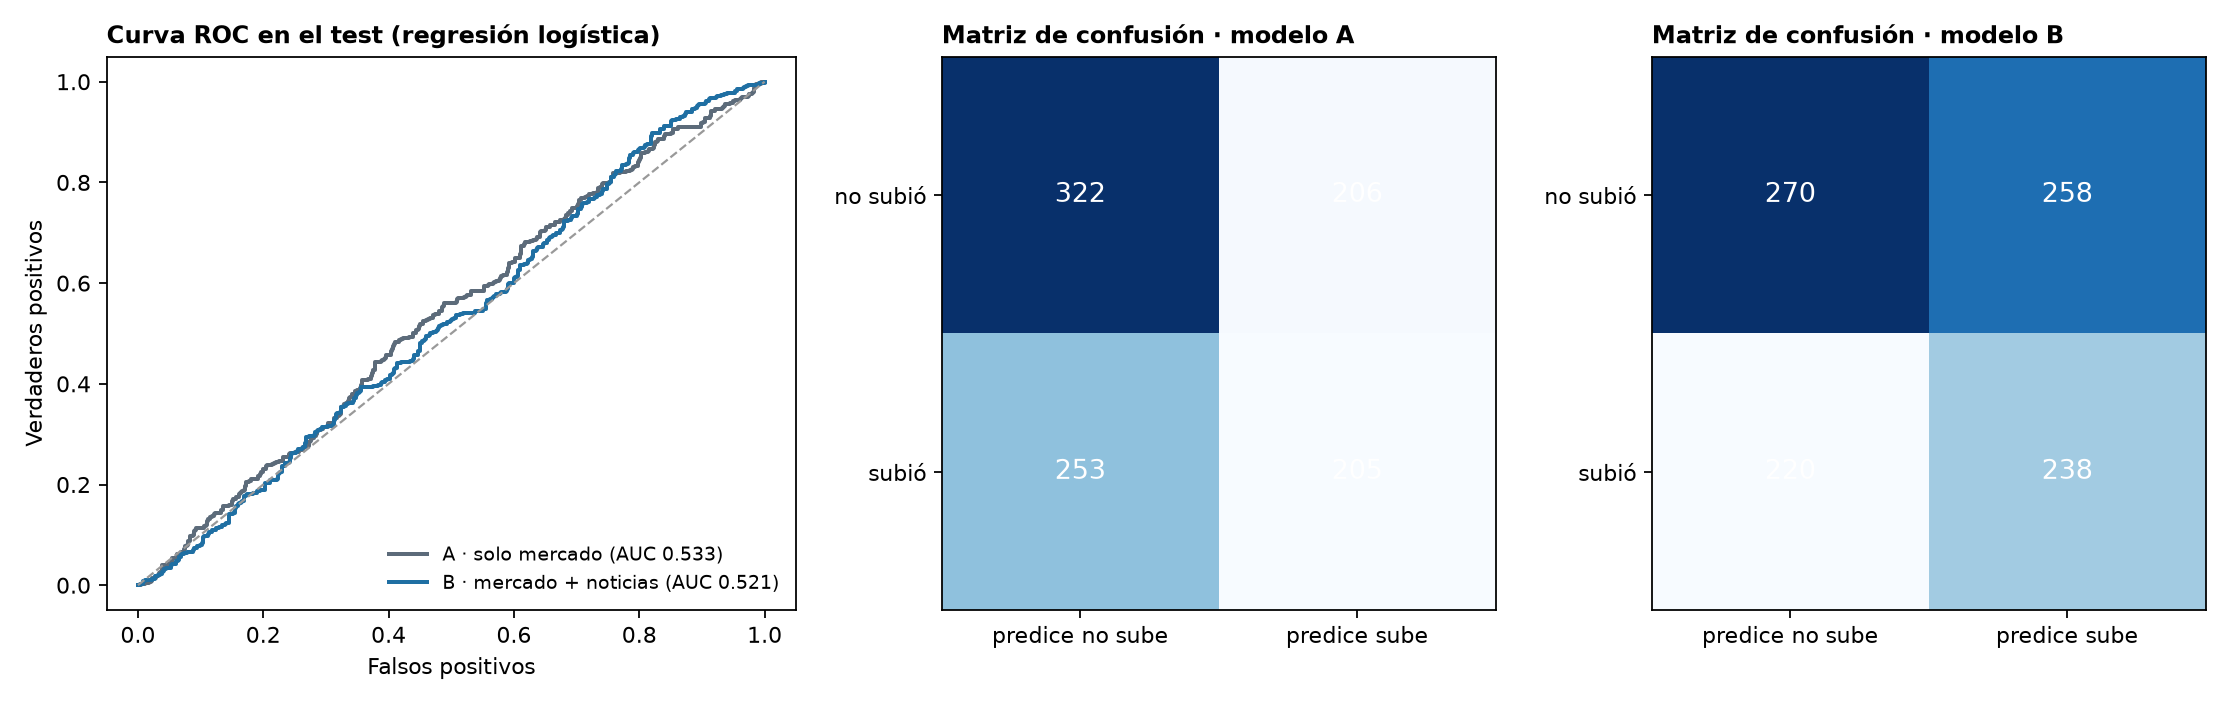
\includegraphics[width=\linewidth]{noticias_a_precio.png}
\caption{Noticias \flecha{} precio, regresión logística. Izquierda: curva ROC de los dos modelos en
el test; las dos van pegadas a la diagonal, que es el azar. Centro y derecha: matrices de confusión.
Fuente: elaboración propia (\carpeta{4_modelado/noticias_a_precio}).}
\label{fig:res-np}
\end{figure}

% ---------------------------------------------------------------------
\section{Precio \flecha{} sentimiento}
\label{sec:res-ps}

\textbf{El mercado sí mejora la predicción del sentimiento de las noticias.} Con solo el pasado de
las noticias, el modelo A predice si el sentimiento de mañana será más positivo que lo habitual con
un AUC de \dato{ps.m.logistica.A.auc@3}, casi el azar. Al agregar el retorno del Merval y el VIX, el
modelo B sube a \textbf{\dato{ps.m.logistica.B.auc@3}} (tabla~\ref{tab:res-ps}):
$\Delta\text{AUC} = \textbf{\dato{ps.d.logistica.delta_auc@s3}}$, con un intervalo del 95\% de
[\dato{ps.d.logistica.ic95_inf@s3};\ \dato{ps.d.logistica.ic95_sup@s3}], que queda entero por
encima de 0. El random forest lo confirma: $\Delta\text{AUC} = \dato{ps.d.random_forest.delta_auc@s3}$
[\dato{ps.d.random_forest.ic95_inf@s3};\ \dato{ps.d.random_forest.ic95_sup@s3}].

\begin{table}[H]
\centering\small
\begin{tabular}{@{}llcccc@{}}
\toprule
\textbf{Algoritmo} & \textbf{Modelo} & \textbf{AUC} & \textbf{Balanced acc.} & \textbf{F1} & \textbf{Exactitud} \\
\midrule
\tabla{metricas_ps}
\bottomrule
\end{tabular}
\caption{Precio \flecha{} sentimiento: métricas en el test (\dato{ps.ruedas_test} ruedas). Modelo A:
solo el pasado de las noticias; modelo B: noticias más mercado. Fuente: elaboración propia
(\carpeta{4_modelado/precio_a_sentimiento}).}
\label{tab:res-ps}
\end{table}

\begin{figure}[H]
\centering
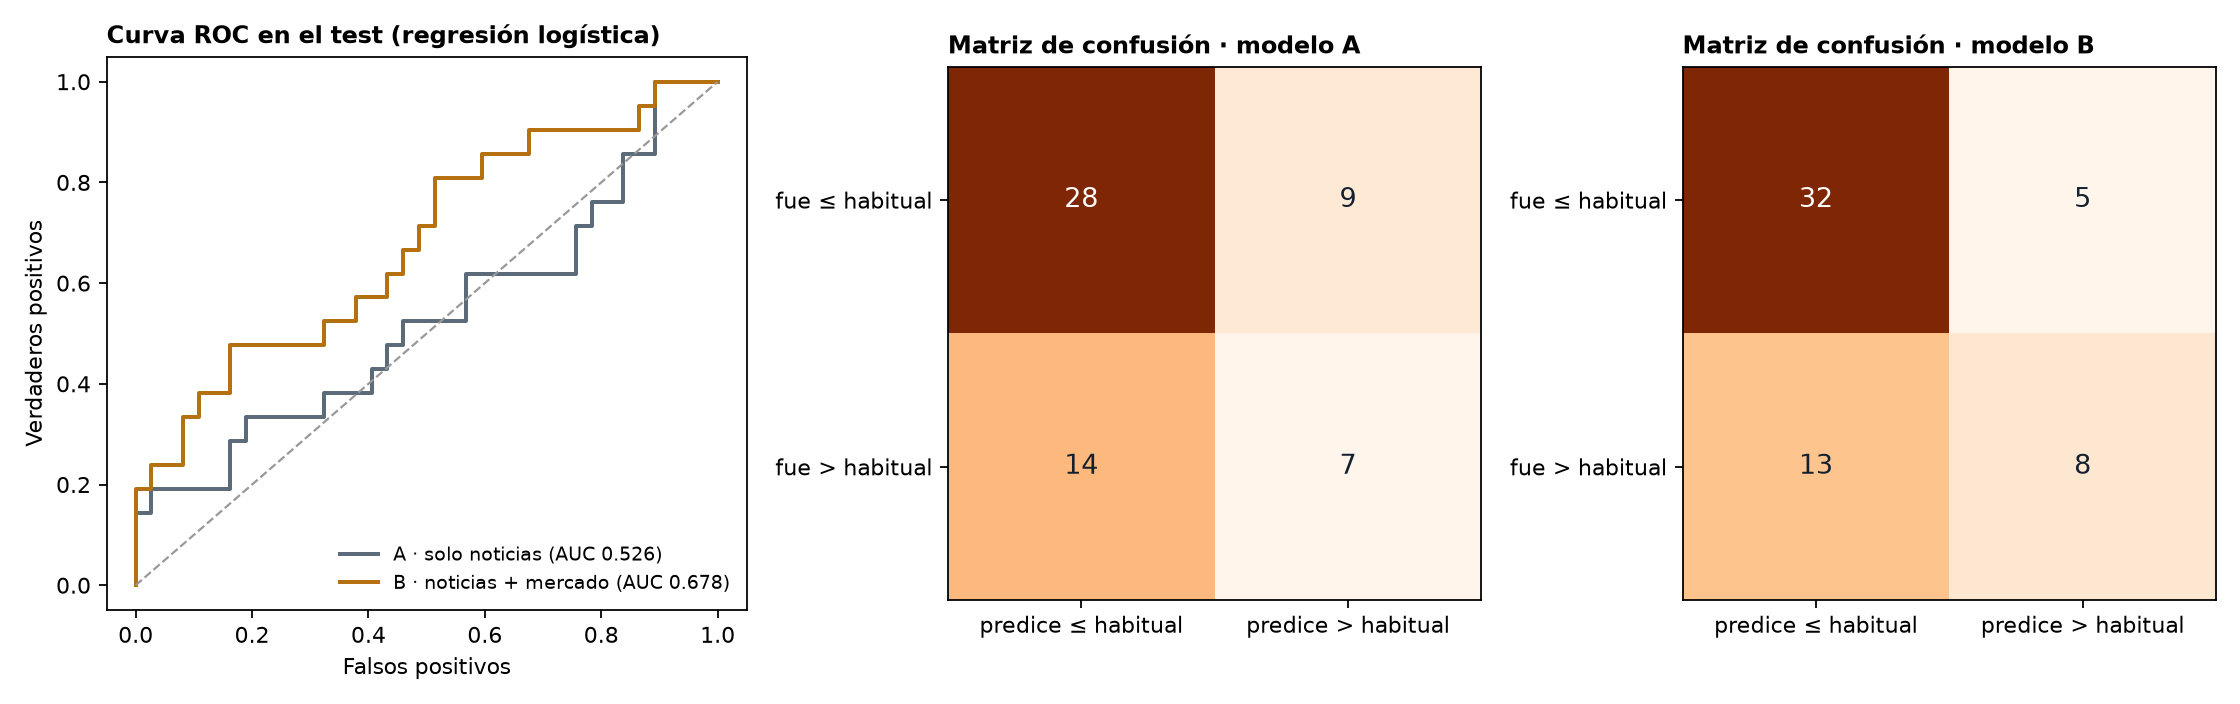
\includegraphics[width=\linewidth]{precio_a_sentimiento.png}
\caption{Precio \flecha{} sentimiento, regresión logística. Izquierda: curva ROC; el modelo B se
separa de la diagonal. Centro y derecha: matrices de confusión. Fuente: elaboración propia
(\carpeta{4_modelado/precio_a_sentimiento}).}
\label{fig:res-ps}
\end{figure}

\textbf{Qué variable pesa.} En el modelo B, la variable con el coeficiente más grande es el
\textbf{retorno del Merval del mismo día} (coeficiente estandarizado
\dato{ps.coef.B.ret_merval_t0@s3}), seguida por el sentimiento inesperado de hoy
(\dato{ps.coef.B.inesperado_t0@s3}) y el retorno de la rueda anterior
(\dato{ps.coef.B.ret_merval_t1@s3}). El signo es positivo: \textbf{cuando el mercado sube hoy, las
noticias de mañana son más positivas que lo habitual}. Por la regla de las 17:00, las noticias de
mañana incluyen las publicadas esta noche, después del cierre: las que cuentan cómo cerró el
mercado.

\textbf{Una lectura de la matriz.} En el test, el sentimiento fue más positivo que lo habitual en
menos ruedas que en el entrenamiento (\dato{ps.m.logistica.B.pct_clase_1_real@pct1}\% contra
\dato{ps.pct_clase_1_entrenamiento@pct1}\%). Con el umbral fijo de 0,5, el modelo B predice la
clase 1 en pocas ruedas, por lo que su F1 es moderado (\dato{ps.m.logistica.B.f1@3}). El AUC, que
no depende del umbral, es la métrica que corresponde para comparar A y B.

% ---------------------------------------------------------------------
\section{Robustez}
\label{sec:robustez}

¿El resultado depende de alguna decisión del diseño? Para responderlo se repitió la comparación
cambiando \textbf{una sola decisión por vez}, en nueve variantes (tabla~\ref{tab:robustez} y
figura~\ref{fig:robustez}). Las variantes se fijaron antes de ver los resultados, salvo «sin abril
de 2026», que se agregó al notar que abril, el mes sin notas de iProfesional, cae dentro del test.

\begin{table}[H]
\centering\footnotesize
\begin{tabular}{@{}lcc@{}}
\toprule
\textbf{Variante} & \textbf{Noticias \flecha{} precio} & \textbf{Precio \flecha{} sentimiento} \\
\midrule
\tabla{robustez}
\bottomrule
\end{tabular}
\caption{Robustez: $\Delta$AUC (B $-$ A) con su intervalo del 95\%, regresión logística. En
negrita, los intervalos que quedan enteros por encima de 0. Fuente: elaboración propia
(\carpeta{5_evaluacion/anexo}).}
\label{tab:robustez}
\end{table}

\begin{figure}[H]
\centering
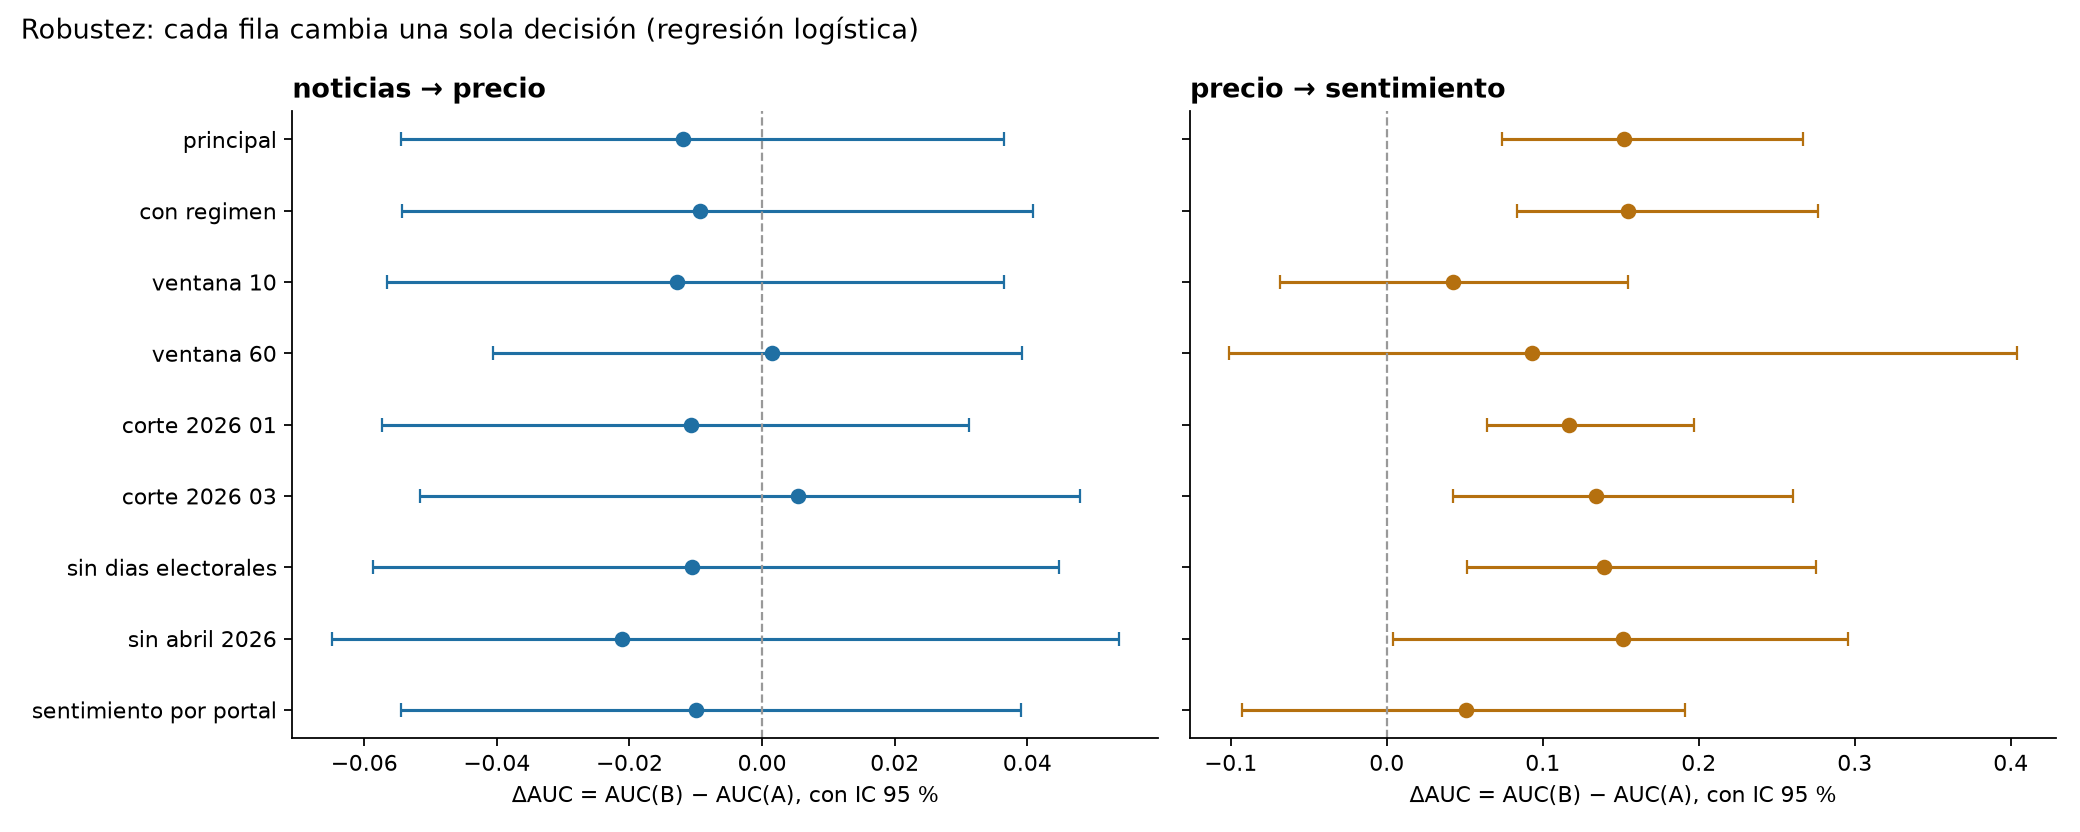
\includegraphics[width=0.94\linewidth]{robustez.png}
\caption{Robustez: cada punto es el $\Delta$AUC de una variante, con su intervalo del 95\%. La línea
discontinua es el 0. Fuente: elaboración propia (\carpeta{5_evaluacion/anexo}).}
\label{fig:robustez}
\end{figure}

\begin{itemize}
  \item \textbf{Noticias \flecha{} precio:} no aporta en \textbf{ninguna} de las variantes
        (\dato{rob.noticias_a_precio_variantes_que_aportan_logistica} con regresión logística y
        \dato{rob.noticias_a_precio_variantes_que_aportan_rf} con random forest). Es el resultado
        más estable del trabajo.
  \item \textbf{Precio \flecha{} sentimiento:} el $\Delta$AUC es \textbf{positivo en las nueve
        variantes}, entre \dato{rob.precio_a_sentimiento_delta_auc_min_logistica@s3} y
        \dato{rob.precio_a_sentimiento_delta_auc_max_logistica@s3}, y su intervalo excluye el 0 en
        \dato{rob.precio_a_sentimiento_variantes_que_aportan_logistica} (con random forest, en
        \dato{rob.precio_a_sentimiento_variantes_que_aportan_rf}). Sobrevive al régimen, a otros
        dos cortes del test, a sacar los días electorales y a sacar abril de 2026. No alcanza en
        tres casos:
        \begin{itemize}
          \item con una ventana de \textbf{10 ruedas}, porque el «habitual» de dos semanas es más
                ruidoso y el objetivo se vuelve más difícil de predecir;
          \item con una ventana de \textbf{60 ruedas}, porque se pierden las primeras 60 ruedas y
                quedan \dato{rob.ventana_60.ps.logistica.filas_entrenamiento} para entrenar: el
                intervalo es muy ancho;
          \item con el \textbf{sentimiento ajustado por portal}, que se discute en la
                sección~\ref{sec:limites}.
        \end{itemize}
\end{itemize}

% ---------------------------------------------------------------------
\section{Verificación clásica: VAR y Granger}
\label{sec:verificacion}

Como verificación, se repitió la pregunta con la econometría clásica: modelos VAR sobre las
\dato{rueda.ruedas_con_inesperado} ruedas con sentimiento inesperado, a nivel mercado y para cada
una de las \dato{dataset.empresas} empresas, con los rezagos elegidos por el criterio de Akaike y
pruebas de causalidad de Granger en las dos direcciones (tabla~\ref{tab:granger}). Los
\dato{var.modelos} VAR son estables.

\begin{table}[H]
\centering\small
\begin{tabular}{@{}lcc@{}}
\toprule
\textbf{Prueba de Granger} & \textbf{Mercado (p)} & \textbf{Empresas con p < 0,05} \\
\midrule
\tabla{granger}
\bottomrule
\end{tabular}
\caption{Causalidad de Granger. Por azar se esperaría que menos de una empresa de
\dato{dataset.empresas} diera p < 0,05. Fuente: elaboración propia (\carpeta{5_evaluacion/anexo}).}
\label{tab:granger}
\end{table}

Los dos métodos dicen lo mismo. El sentimiento no anticipa el retorno del Merval
(p~=~\dato{var.mercado.ines_ret.p}) ni el de ninguna empresa. El retorno sí anticipa el sentimiento:
en el mercado (p~\dato{var.mercado.ret_ines.p}) y en \dato{var.emp.ret_ines.sig} de las
\dato{dataset.empresas} empresas, todas con efecto positivo. En la función de impulso-respuesta,
una suba de un desvío del Merval hace subir el sentimiento de la rueda siguiente
\dato{var.irf.ret_ines.h1.irf@1} puntos (banda del 95\%: \dato{var.irf.ret_ines.h1.banda_baja@1} a
\dato{var.irf.ret_ines.h1.banda_alta@1}). Lo mismo pasa con el sentimiento propio de cada empresa:
después de que su acción sube, se habla de ella mejor que del resto del mercado
(\dato{var.emp.ret_prop.sig} de \dato{dataset.empresas}).

\begin{figure}[H]
\centering
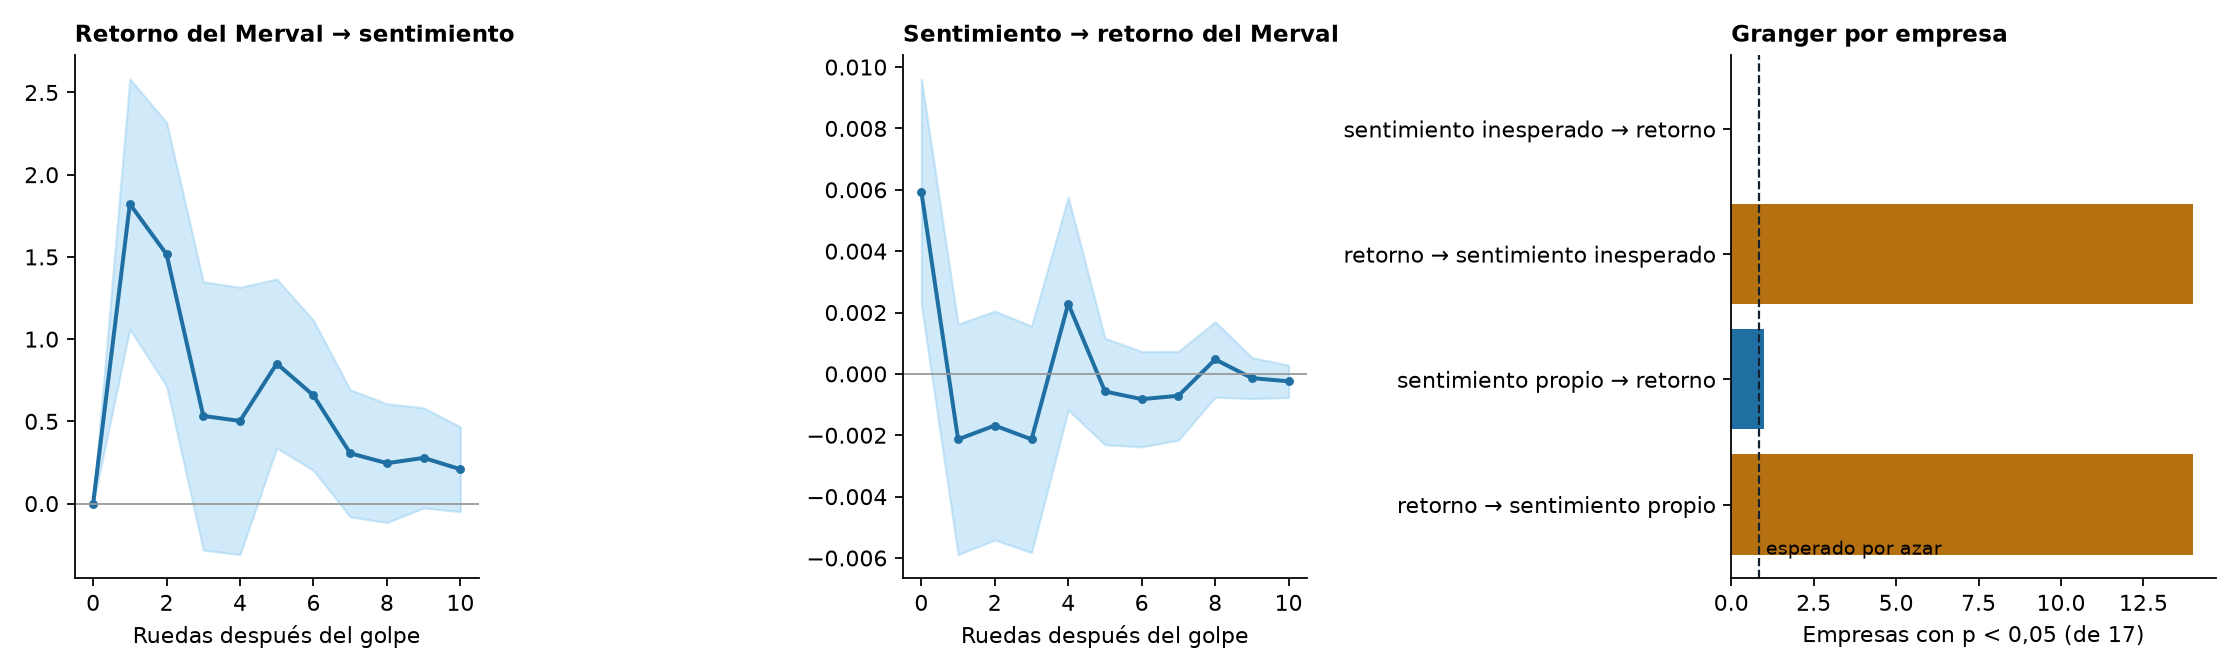
\includegraphics[width=\linewidth]{var_granger.png}
\caption{Verificación clásica. Izquierda y centro: impulso-respuesta del mercado, con banda del
95\%. Derecha: empresas con p < 0,05 en cada prueba de Granger; la línea discontinua es lo esperado
por azar. Fuente: elaboración propia (\carpeta{5_evaluacion/anexo}).}
\label{fig:granger}
\end{figure}

% ---------------------------------------------------------------------
\section{Veredicto}
\label{sec:veredicto}

La tabla~\ref{tab:veredicto} aplica el criterio de aceptación de la sección~\ref{sec:hipotesis},
fijado antes de ver los resultados.

\begin{table}[H]
\centering\small
\begin{tabularx}{\linewidth}{@{}L{4.2cm}YC{1.8cm}@{}}
\toprule
\textbf{Parte del criterio} & \textbf{Resultado} & \textbf{¿Cumple?} \\
\midrule
1. FinBETO supera al modelo de referencia & F1 macro \dato{fb.f1_macro_media@3} contra \dato{fbcmp.completo.referencia_f1_macro@3} (\dato{fbcmp.completo.ventaja_puntos} puntos más) & Sí \\
2a. Noticias \flecha{} precio & $\Delta$AUC \dato{np.d.logistica.delta_auc@s3} [\dato{np.d.logistica.ic95_inf@s3}; \dato{np.d.logistica.ic95_sup@s3}] & No \\
2b. Precio \flecha{} sentimiento & $\Delta$AUC \dato{ps.d.logistica.delta_auc@s3} [\dato{ps.d.logistica.ic95_inf@s3}; \dato{ps.d.logistica.ic95_sup@s3}] & Sí \\
2. Al menos una dirección & Precio \flecha{} sentimiento & Sí \\
\midrule
\textbf{Veredicto} & \multicolumn{2}{l}{\textbf{Se rechaza H0: se acepta H1}} \\
\bottomrule
\end{tabularx}
\caption{Veredicto sobre la hipótesis. Fuente: elaboración propia
(\carpeta{5_evaluacion/veredicto_hipotesis}).}
\label{tab:veredicto}
\end{table}

\textbf{Se rechaza H0.} La metodología \textit{mide} el sentimiento de la prensa económica argentina
mejor que un modelo genérico, y lo \textit{relaciona} con el mercado. La relación va en una sola
dirección: \textbf{el mercado anticipa al sentimiento de los medios, no al revés}.
